\documentclass[titlepage,letterpaper,final,11pt]{scrartcl}

\usepackage[total={6.0in,8.75in},top=1.2in,left=1.35in]{geometry}

% this lets us avoid the scrartcl/hyperref conflict...
%\let\ifvtex\relax

\usepackage{verbatim}
\usepackage{empheq}
\usepackage{color}
\usepackage{animate}
\usepackage{graphicx}

% hyperref should be the last package we load
\usepackage[pdftex,
colorlinks=true,
plainpages=false, % only if colorlinks=true
linkcolor=blue,   % only if colorlinks=true
citecolor=blue,   % only if colorlinks=true
urlcolor=blue     % only if colorlinks=true
]{hyperref}

\pdfinfo{
/Title (Numerical modelling of ice sheets, streams, and shelves)
/Author (Ed Bueler)
/Subject (numerical modelling of glaciers, ice sheets, and ice shelves)
/Keywords (numerical model, numerical analysis, glacier, ice sheet, ice shelf, shallow models of ice flow)
}

\newcommand{\ddt}[1]{\ensuremath{\frac{\partial #1}{\partial t}}}
\newcommand{\ddx}[1]{\ensuremath{\frac{\partial #1}{\partial x}}}
\newcommand{\ddy}[1]{\ensuremath{\frac{\partial #1}{\partial y}}}
\newcommand{\pp}[2]{\ensuremath{\frac{\partial #1}{\partial #2}}}
\renewcommand{\t}[1]{\texttt{#1}}
\newcommand{\Matlab}{\textsc{Matlab}\xspace}
\newcommand{\bq}{\mathbf{q}}
\newcommand{\bU}{\mathbf{U}}
\newcommand{\eps}{\epsilon}
\newcommand{\grad}{\nabla}
\newcommand{\Div}{\nabla\cdot}
\newcommand{\devstress}{\tau}

\newcommand{\mname}[1]{\href{http://www.dms.uaf.edu/~bueler/mccarthy/mfiles/#1}{\texttt{#1}}}

\newcommand{\txtinput}[1]{\scriptsize\verbatiminput{#1}}

\newcommand{\txtinputtiny}[1]{\tiny\verbatiminput{#1}}

\newcommand{\mmessage}[1]{\begin{center}
\emph{see code} \url{http://www.dms.uaf.edu/~bueler/mccarthy/mfiles/#1.m}
\end{center}}

\newcommand{\mmess}[1]{\vspace{-0.1in}\begin{center}
\fbox{\url{http://www.dms.uaf.edu/~bueler/mccarthy/mfiles/#1.m}}
\end{center}}

\newcommand{\minput}[1]{\scriptsize\verbatiminput{mfiles/#1.slim.m}
\tiny\mmess{#1}\normalsize}

\newcommand{\minputtiny}[1]{\tiny\verbatiminput{mfiles/#1.slim.m}
\mmess{#1}\normalsize}

\newcommand{\alert}[1]{\emph{#1}}



\begin{document}
\graphicspath{{../photos/}{../pdffigs/}}
%\addgraphicspath{{{../pdffigs/}}


\begin{titlepage}

  \begin{center}
    {\Large\usekomafont{title} Numerical modelling of ice sheets, streams, and shelves}
    \vspace{0.5cm}

    {\large Ed Bueler}
    \vspace{1cm}

    September 2012
    %\includegraphics[width=3.3in,keepaspectratio=true]{grn-1km-csurf} \vfill
  \end{center}
\end{titlepage}


\section{preamble}

slogans:
  \begin{enumerate}
  \item \alert{focus on approximating ice flow}
  \item \alert{example numerical codes that actually work}
  \end{enumerate}
\medskip

scope:
  \begin{itemize}
  \item[$\circ$] continuum models

    \begin{itemize}
    \item shallow ice approximation (SIA) in 2D
    \item shallow shelf approximation (SSA) in 1D
    \item mass continuity \& surface kinematical equations
    \end{itemize}

  \item[$\circ$] numerical ideas

    \begin{itemize}
    \item finite difference schemes
    \item solving algebraic systems from stress balances
    \item verification
    \end{itemize}
  \end{itemize}



\emph{not} \normalsize covered here:

  \begin{itemize}
  \item Stokes and ``higher order'' flow equations
  \item thermomechanical coupling or polythermal ice
  \item subglacial hydrology/processes
  \item mass balance and snow/firn processes
  \item constitutive relations other than Glen isotropic
  \item grounding lines, calving fronts, ocean interaction
  \item paleo-climate and ``spin-up''
  \item earth deformation under ice sheet load
  \item other numerics: FEM, spectral, multigrid, parallel, \dots
  \item etc.
  \end{itemize}


\begin{center}
  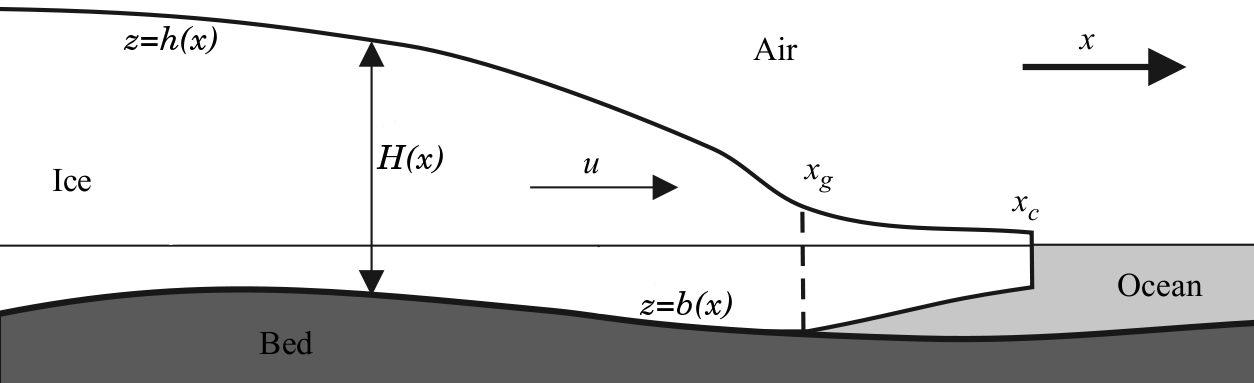
\includegraphics[width=5.0in]{flowline}

\emph{figure modified from} Schoof (2007)\nocite{SchoofMarine1}
\end{center}

  \begin{itemize}
  \item coordinates $t,x,y,z$  (with $z$ vertical, positive upward)
  \item subscripts for partial derivatives $u_x = \partial u/\partial x$
  \item $H=$ ice thickness
  \item $h=$ ice surface elevation
  \item $b=$ bedrock surface elevation
  \item $T=$ ice temperature
  \item $\mathbf{u}=(u,v,w)=$ ice velocity
  \item $\rho=$ density of ice
  \item $\rho_w=$ density of ocean water
  \item $g=$ acceleration of gravity
  \item $n=3$ Glen flow law exponent $=3$
  \item $A=A(T)=$ ice softness in Glen law ($\mathbf{D}_{ij} = A(T) \tau^{n-1} \tau_{ij}$)
  \item \alert{please ask about notation!}  (stupid questions impossible)
  \end{itemize}

%notation generally consistent with these references
\nocite{BLKCB,BBssasliding,Fowler,GreveBlatter2009,SchoofStream,SchoofMarine1}

Matlab/Octave codes:

\begin{itemize}
\item lectures are structured around 14 ice flow codes
\item each is $\sim$ 1/2 page of Matlab/Octave code
\item \texttt{.zip} and \texttt{.tar.gz} forms available from memory stick
\item online:

\centerline{\fbox{\url{http://www.dms.uaf.edu/~bueler/mccarthy/mfiles/}}}
\end{itemize}


\subsection{ice flow equations}


my first goal

\begin{itemize}
\item my goal is to get to an equation for which I can say:

\begin{center}
\emph{numerically solve just this equation, and you've got a usable model for a flowing ice sheet}
\end{center}

\item to get to my goal I will quickly recall the continuum mechanics of ice flow
\item a ``usable'' model is \emph{understood} more than it is \emph{correct}
\end{itemize}


ice in glaciers is a \emph{fluid}

\begin{itemize}
\item we describe fluids primarily by a \emph{velocity field} $\mathbf{u}(t,x,y,z)$
\item if ice fluid were
  \begin{itemize}
  \item[$\circ$] faster-moving than it actually is (e.g.: gravity stronger?), and
  \item[$\circ$] linearly-viscous like liquid water
  \end{itemize}
  
  then ice flow would be a more-familiar, ``typical'' fluid
\item in that case we would all use the Navier-Stokes equations as our flow model:
\begin{align*}
\nabla \cdot \mathbf{u} &= 0 &&\text{\emph{incompressibility}} \\
\rho \left(\mathbf{u}_t + \mathbf{u}\cdot\nabla \mathbf{u}\right) &= -\nabla p + \nu \nabla^2 \mathbf{u} + \rho \mathbf{g} &&\text{\emph{force balance}}
\end{align*}
\end{itemize}


\emph{hmmm} \dots \emph{does not sound like glaciology to me!}

is numerical ice flow modeling a part of computational fluid dynamics?

\begin{itemize}
\item \alert{yes}
\item large scale like atmosphere/ocean
\item \dots but it is a weird one
\item consider what makes atmosphere/ocean flow modeling exciting:
  \begin{itemize}
  \item[$\circ$] turbulence
  \item[$\circ$] convection
  \item[$\circ$] coriolis force
  \item[$\circ$] density/salinity variation
  \item[$\circ$] chemistry (methane, ozone, \dots)
  \end{itemize}
\item none of the above list is relevant to ice flow
\item so what could be interesting about the flow of slow, cold, stiff, laminar, inert old ice?

 \qquad \dots \qquad it's \emph{ice dynamics!}
\end{itemize}


ice is a slow, shear-thinning fluid

\begin{itemize}
\item our fluid is

  \begin{tabular}{lc}
  \emph{slow}: & $\rho \left(\mathbf{u}_t + \mathbf{u}\cdot\nabla \mathbf{u}\right) \approx 0$ \\
  \emph{non-Newtonian}: & viscosity $\nu$ is not constant
  \end{tabular}
\item ``shear-thinning'' flow: bigger strain rate means smaller viscosity
\item the standard ``full'' model is Glen-law ($n=3$) Stokes:
\begin{align*}
\nabla \cdot \mathbf{u} &= 0 &&\text{\emph{incompressibility}} \\
0 &= - \nabla p + \nabla \cdot \tau_{ij} + \rho \mathbf{g} &&\text{\emph{force balance}} \\
\mathbf{D}_{ij} &= A \tau^2 \tau_{ij} &&\text{\emph{flow law}}
\end{align*}
\item these equations above are true at every instant, and
  \begin{quote}
  \emph{geometry, boundary stress, and ice viscosity determine velocity instantaneously}
  \end{quote}
\end{itemize}


\begin{itemize}
\item ``slow'':
  $$\rho \left(\mathbf{u}_t + \mathbf{u}\cdot\nabla \mathbf{u}\right) \approx 0 \qquad \iff \qquad \begin{pmatrix} \text{forces of inertia} \\ \text{are negligible} \end{pmatrix}$$
\item a time-stepping ice sheet code recomputes the full velocity field at every time step, without requiring velocity from the previous step\footnote{to be a weatherman you've got to know which way the wind blows \dots but don't expect that from a glaciologist}
\item thus no memory of previous momentum/velocity, so
  \begin{quote}\emph{velocity is a ``diagnostic'' output of an ice flow model}\end{quote}
\end{itemize}

plane flow Stokes:

\begin{itemize}
\item in the $x,z$ plane flow case the Stokes equations say
\begin{empheq}[]{align}
u_x + w_z &= 0 &&\text{\emph{incompressibility}}\notag \\
p_x &= \tau_{11,x} + \tau_{13,z} &&\text{\emph{stress balance} ($x$)} \notag \\
p_z &= \tau_{13,x} - \tau_{11,z} - \rho g &&\text{\emph{stress balance} ($z$)} \notag \\
u_x &= A \tau^2 \tau_{11} &&\text{\emph{flow law} (diagonal)}\notag \\
u_z + w _x &= 2 A \tau^2 \tau_{13} &&\text{\emph{flow law} (off-diagonal)} \notag
\end{empheq}
\item $x,z$ subscripts are partial derivatives
\item $\tau_{13}$ is a ``vertical'' shear stress
\item $\tau_{11}$ and $\tau_{33}=-\tau_{11}$ are deviatoric longitudinal stresses 
\item we have five equations in five unknowns ($u,w,p,\tau_{11},\tau_{13}$)
\item complicated enough \dots what about in a simplified situation?
\end{itemize}


\subsection{slab-on-a-slope}

\begin{itemize}
\item rotated coordinates:
  $$\mathbf{g} = g \sin\theta\, \hat x - g \cos \theta \,\hat z$$
\item so $p_x,p_z$ equations are now:
\begin{align}
p_x &= \tau_{11,x} + \tau_{13,z} + \rho g \sin\theta \notag \\
p_z &= \tau_{13,x} - \tau_{11,z} - \rho g \cos\theta \notag
\end{align}
\end{itemize}

\begin{center}
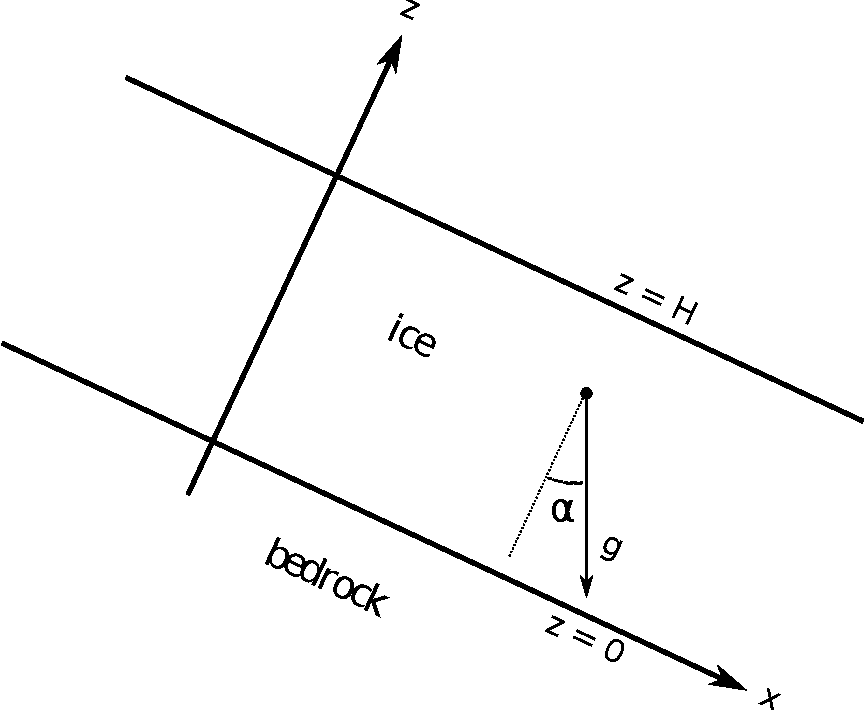
\includegraphics[width=3.0in]{slab}
\end{center}

\begin{itemize}
\item for a slab-on-a-slope there is \emph{no variation in} $x$
\item so equations simplify:
\begin{empheq}[box=\fbox]{align}
w_z &= 0 &   0 &= \tau_{11} \notag \\
\tau_{13,z} &= - \rho g \sin\theta &   u_z &= 2 A \tau^2 \tau_{13} \notag \\
p_z &= - \rho g \cos\theta \notag
\end{empheq}
\end{itemize}


\begin{itemize}
\item add some boundary conditions:
	$$w(\text{base})=0, \qquad p(\text{surface})=0, \qquad u(\text{base})=u_0$$
\item by integrating vertically, get :
  $$w=0, \qquad p = \rho g \cos\theta (H-z), \qquad \tau_{13} = \rho g \sin\theta (H-z)$$
\item and from ``$u_z = 2 A \tau^2 \tau_{13}$'' get
\vspace{-0.05in}
\begin{align*}
u(z) &= u_0 + 2 A (\rho g \sin\theta)^3 \int_0^z (H-z')^3\,dz' \\
     &= u_0 + \frac{1}{2} A (\rho g \sin\theta)^3  \left(H^4 - (H-z)^4\right)
\end{align*}
\end{itemize}

\begin{center}
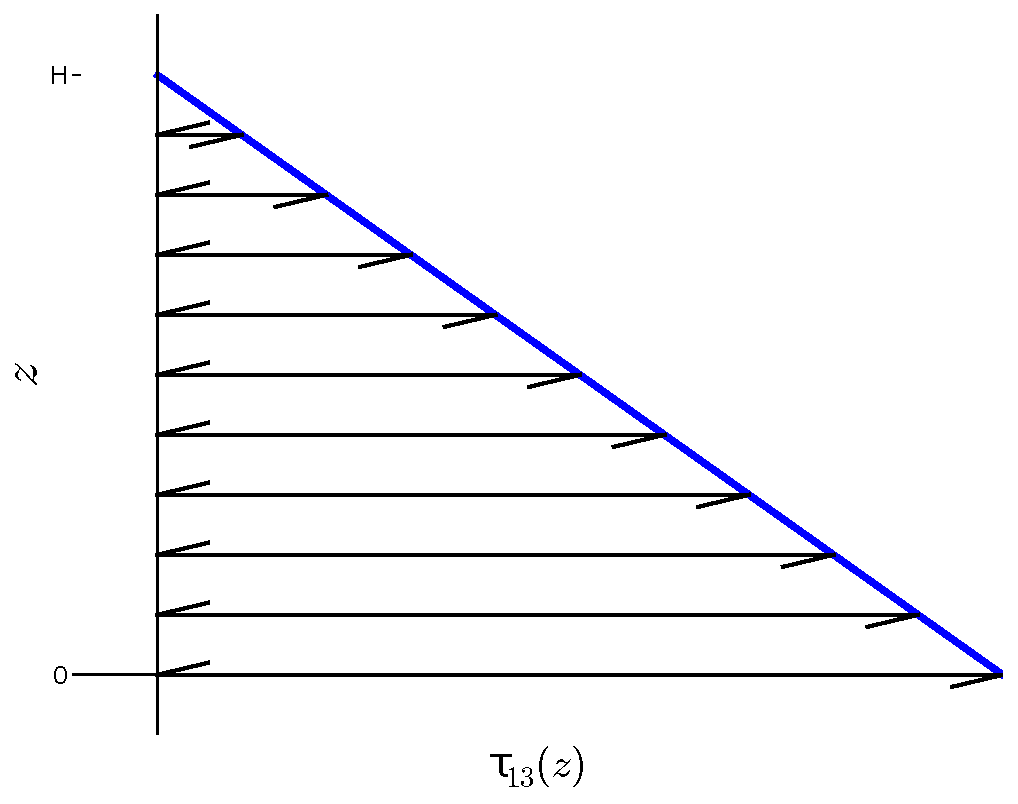
\includegraphics[width=3.0in]{slabshear}
\end{center}


\begin{itemize}
\item do we believe these equations?
\item velocity on last slide (and below) was from a \emph{formula}
\item compare to observations at right
\end{itemize}


\begin{center}
% NOT preserving aspect ratio
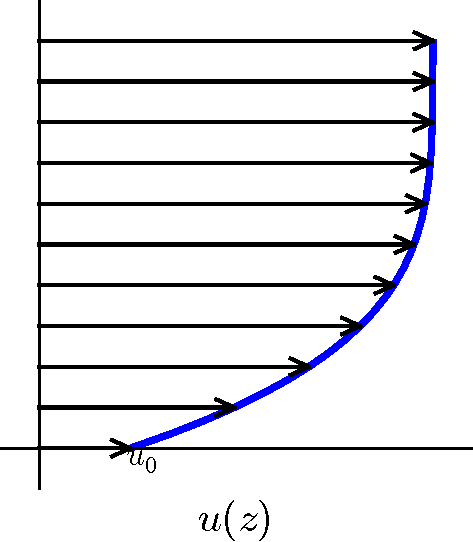
\includegraphics[width=2.5in]{slabvel}
\quad
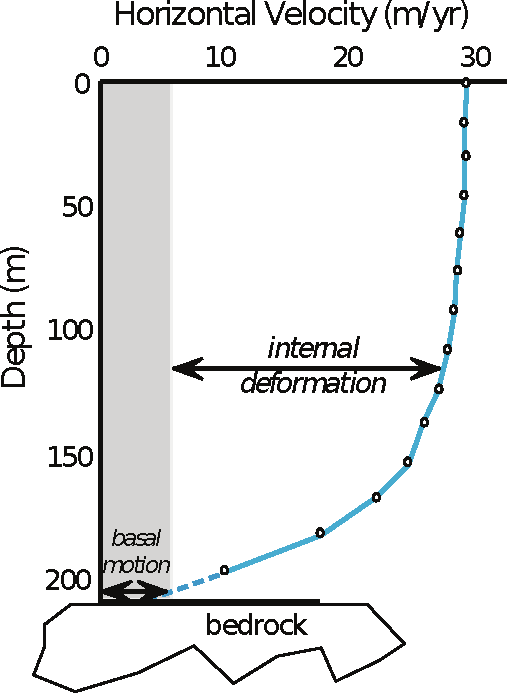
\includegraphics[width=2.5in]{athabasca_deform}
\end{center}


Velocity profile of the Athabasca Glacier, Canada, derived from inclinometry (Savage and Paterson, 1963)\nocite{SavagePaterson}


mass continuity:

\begin{itemize}
\item now we know the velocity $u=u(t,x,z)$ \dots so what?
\item suppose our slab has variable thickness $H(t,x)$
\item compute the vertical average of velocity:
	$$\bar u(x,t) = \frac{1}{H}\int_0^{H} u(t,x,z)\,dz$$
\end{itemize}

\begin{itemize}
\item consider change of area (ice volume in 3D) in the figure:
	$$\frac{dA}{dt} = \int_{x_1}^{x_2} M(x)\,dx + \bar u_1 H_1 - \bar u_2 H_2$$
\item but, assuming width $dx=x_2-x_2$ is small, $A\approx dx\, H$; divide by $dx$ and get
   $$H_t = M - \left(\bar u H\right)_x$$
\item this is a \emph{mass continuity equation}
\item I'll return to this topic \dots
\end{itemize}

\begin{center}
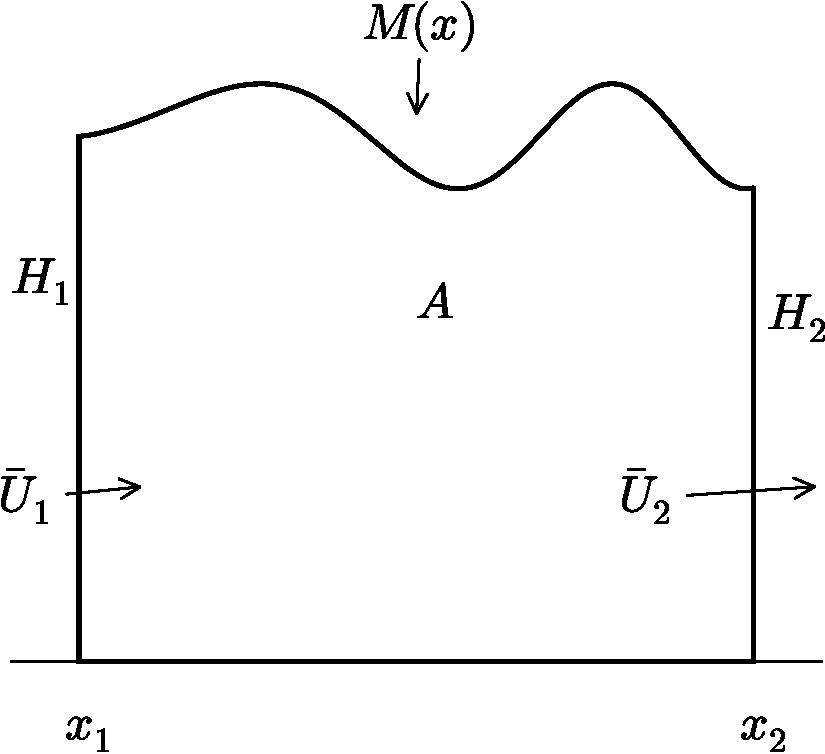
\includegraphics[width=2.5in]{slabmasscontfig}
\quad
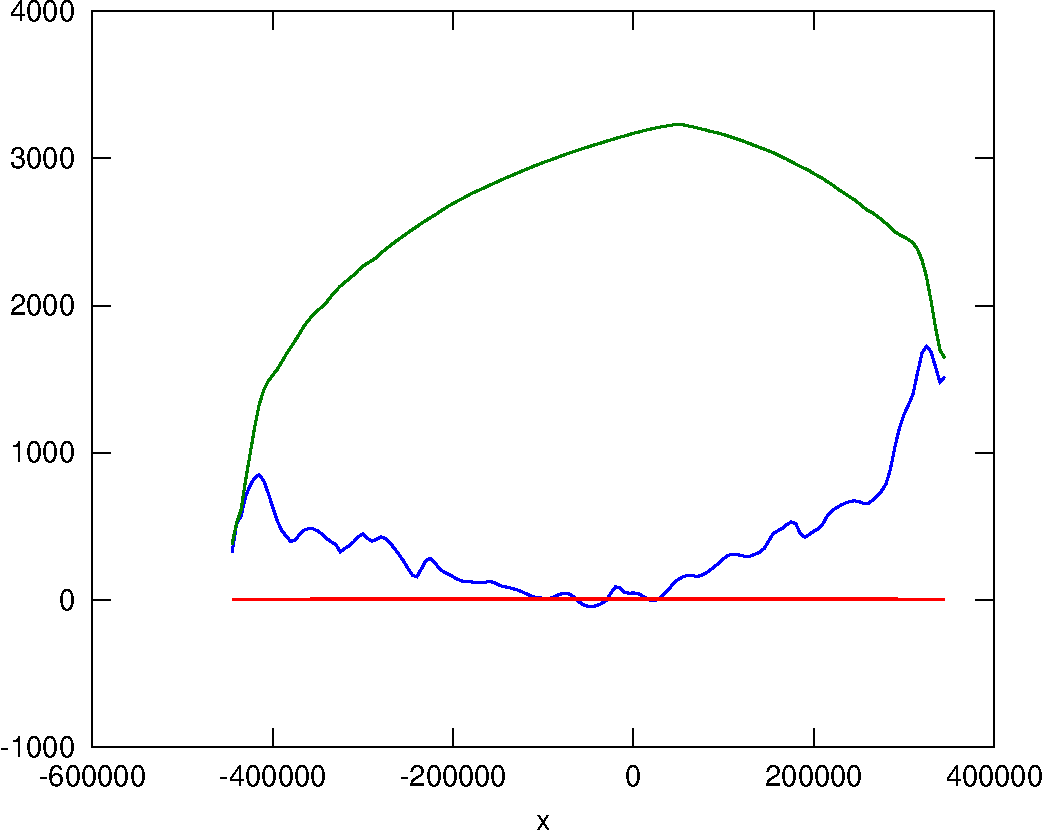
\includegraphics[width=2.5in]{green_transect}
\end{center}


rough explanation of ``shallow ice approximation'' (SIA)

\begin{itemize}
\item from slab-on-slope velocity formula in $u_0=0$ case (``non-sliding SIA''),
\begin{align*}
\bar u H &= \int_0^H \frac{1}{2} A (\rho g \sin\theta)^3  \left(H^4 - (H-z)^4\right)\,dz \\
	&= \frac{1}{2} A (\rho g \sin\theta)^3  \left(\frac{4}{5} H^5\right) \\
	&= \frac{2}{5} A (\rho g \sin\theta)^3 H^5
\end{align*}
\item note $\sin \theta \approx \tan\theta = - h_x$
\item combine with mass continuity $H_t = M - \left(\bar u H\right)_x$:
  $$H_t = M + \left(\frac{2}{5} (\rho g)^5 A H^5 |h_x|^2 h_x\right)_x.$$
\item I'll return to this topic \dots
\end{itemize}



\section{shallow ice sheets}

slow, non-Newtonian, some basal slip, and shallow

\begin{itemize}
\item ice sheets have four outstanding properties \emph{as fluids}:
  \begin{enumerate}
  \item slow
  \item non-Newtonian
  \item contact slip (sometimes)
  \item shallow
  \end{enumerate}
\end{itemize}

regarding ``shallow''

\begin{itemize}
\item below in \alert{red} is a no-vertical-exaggeration cross section of Greenland at $71^\circ$
\small
\item green and blue: standard vertically-exaggerated cross section
\item you can scale Stokes equation using smallness of $\eps = [H]/[L]$, where $[H]$ is a typical thickness of an ice sheet and $[L]$ is a typical horizontal dimension, \dots (Fowler, 1997)\nocite{Fowler}
\end{itemize}


\subsection{shallow ice approx (SIA)}

flow model I: non-sliding, isothermal shallow ice approximation = (SIA)

a model which applies to
\begin{itemize}
\item small depth-to-width ratio (``shallow'') grounded ice sheets
\item on not-too-rough bed topography,
\item whose flow is not dominated by sliding and/or liquid water at the base or margin
\end{itemize}

\begin{center}
  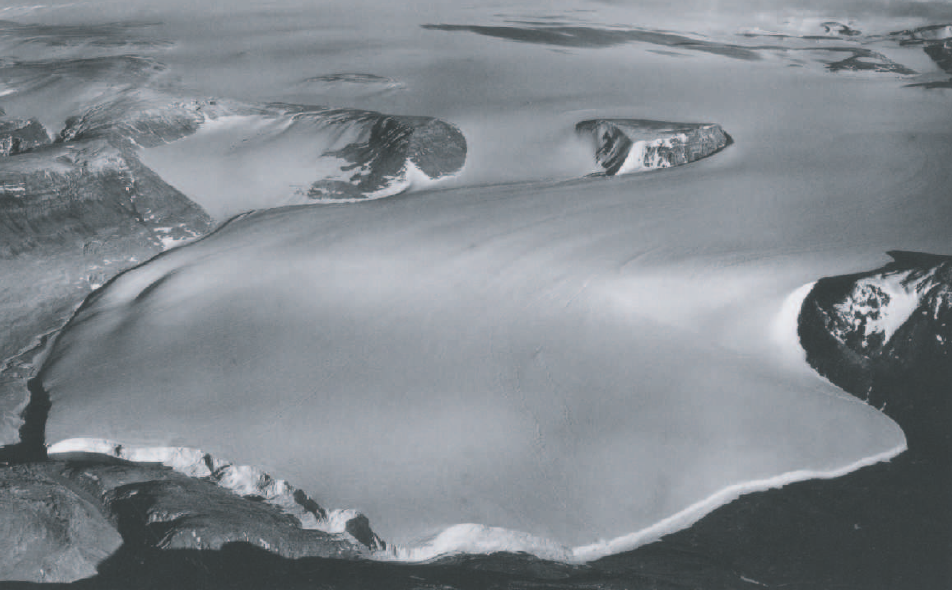
\includegraphics[width=3.0in]{polaris}

``Polaris Glacier,'' northwest Greenland, photo 122, Post \& LaChapelle (2000)\nocite{PostLaChapelle}
\end{center}

SIA model equations

\begin{itemize}
\item though the best explanation of the SIA is to use shallowness to simplify the Stokes equations, here we take the simple slogan:

\begin{center}
\emph{the SIA uses the formulas from slab-on-a-slope}
\end{center}
\item shear stress approximation:
	$$(\tau_{13},\tau_{23}) \approx - \rho g (h-z) \nabla h$$
\item let $\mathbf{u} = (u,v)$, the horizontal velocity
\item we further approximate
\begin{align*}
\mathbf{u}_z &\approx 2 A |(\tau_{13},\tau_{23})|^{n-1} (\tau_{13},\tau_{23}) \\
     &= - 2 A (\rho g)^n (h-z)^n |\nabla h|^{n-1} \nabla h
\end{align*}
\item by integrating vertically, in the non-sliding case,
    $$\mathbf{u} = - \frac{2 A (\rho g)^n}{n+1} \left[H^{n+1} - (h-z)^{n+1}\right] |\nabla h|^{n-1} \nabla h$$
\item but mass continuity remains, $H_t = M - \left(\overline{\mathbf{u}} H\right)_x$
\end{itemize}

SIA thickness equation

\begin{itemize}
\item from last slide, we get the non-sliding, isothermal shallow ice approximation for how thickness changes:
\begin{empheq}[box=\fbox]{equation}
H_t = M + \Div \left(\Gamma H^{n+2} |\grad h|^{n-1} \grad h \right) \label{sia}
\end{empheq}

\vspace{-2mm}
  \begin{itemize}
  \item[$\circ$] where $H$ is ice thickness, $h$ is ice surface elevation, $b$ is bed elevation ($h=H+b$)
  \item[$\circ$] $M$ combines surface and basal mass (im)balance:

     accumulation if $M>0$, ablation if $M<0$
  \item[$\circ$] $n$ is the exponent in the Glen flow law
  \item[$\circ$] $\Gamma = 2 A (\rho g)^n / (n+2)$ is a positive constant
  \end{itemize}
\item numerically solve just equation (1), and you've got a usable model for \dots \emph{the Barnes ice cap} (Mahaffy, 1976)\nocite{Mahaffy}
\end{itemize}
\medskip

\noindent good questions:
\begin{enumerate}
\item where does equation (1) come from?
\item how to solve it numerically?
\item how to \emph{think} about it?
\end{enumerate}


\subsection{analogy w heat equation}

heat equation

\begin{itemize}
\item for understanding SIA, recall heat equation
\item recall Newton's law of cooling
	$$\frac{dT}{dt} = -K (T-T_{\text{ambient}})$$
where $T$ is object temperature and $K$ relates to material and geometry of object (e.g.~cup of coffee)
\item Newton's law for segments of a rod:
\begin{align*}
\frac{dT_j}{dt} &= -K \left(T_j - \frac{1}{2} (T_{j-1} + T_{j+1}) \right) \\
	&= \frac{K}{2} \left(T_{j-1} - 2 T_j + T_{j+1}\right) 
\end{align*}
\item this has limit as segments shrink:
	$$T_t = D T_{xx}$$
\item compare: finite difference approximations to derivatives
\end{itemize}


more complete and 2D version of heat equation

\begin{itemize}
\item $u(t,x,y)$ is temperature in object at position $x,y$ and time $t$
\item Fourier rewrote Newton's law as a rule for heat flux: $\mathbf{q} = - k \grad u$
\item allow an additional heat source $f$
\item coefficients: $\rho$ is density, $c$ is specific heat, $k$ is conductivity
\item by conservation of energy get heat equation:
	$$\rho c u_t = f + \Div (k \grad u)$$
\end{itemize}

\begin{itemize}
\item define the ``diffusivity constant'' $D=k/(\rho c)$ and also $F := f/(\rho c)$
\item for 2D object (e.g.~a plate):
\begin{equation}
u_t = F + \Div (D\, \grad u) \label{heat}
\end{equation}
\item this is like the SIA model for ice sheets: temperature $u$ solves a \emph{diffusive, time-evolving partial differential equation (PDE)}
\end{itemize}

analogy: SIA versus heat equation

\begin{itemize}
\item side-by-side comparison:
\begin{center}
\begin{tabular}{cc}
SIA:\, $H(t,x,y)$ is ice thickness & \scriptsize heat: $u(t,x,y)$ is temperature \\
	\boxed{H_t = M + \Div \left({\color{red}\Gamma H^{n+2} |\grad h|^{n-1}}\, \grad h \right)}  &  \boxed{u_t = F + \Div (D\, \grad u)}
\end{tabular}
\end{center}

\item we identify the diffusivity in the SIA:
	$$D = {\color{red}\Gamma H^{n+2} |\grad h|^{n-1}}$$
\item \emph{non-sliding shallow ice flow \alert{diffuses} the ice sheet}
\item some issues with this analogy:
  \begin{itemize}
  \item[$\circ$]  $D$ depends on solution $H(t,x,y)$
  \item[$\circ$]  $D\to 0$ at margin, where $H\to 0$
  \item[$\circ$]  $D\to 0$ at divides/domes, where $|\grad h|\to 0$
  \end{itemize}
\end{itemize}


\subsection{finite difference numerics}

numerics for heat equation: basic ideas of finite differences

\begin{itemize}
\item numerical schemes for heat equation are good start for SIA
\item for differentiable $f(x)$ and any $h$, \emph{Taylor's theorem} says
	$$f(x+h) = f(x) + f'(x) h + \frac{1}{2} f''(x) h^2 + \frac{1}{3!} f'''(x) h^3 + \dots$$
\item you can replace ``$h$'' by multiples of $\Delta x$, e.g.:
\begin{align*}
f(x-\Delta x) &= f(x) - f'(x) \Delta x + \frac{1}{2} f''(x) \Delta x^2 - \frac{1}{3!} f'''(x) \Delta x^3 + \dots \\
f(x+2\Delta x) &= f(x) + 2 f'(x) \Delta x + 2 f''(x) \Delta x^2 + \frac{4}{3} f'''(x) \Delta x^3 + \dots
\end{align*}
\item \emph{combine expressions like these to give approximations of derivatives, from values on a grid}
\end{itemize}

finite differences for partial derivatives

\begin{itemize}
\item we want partial derivative expressions, for example with $u=u(t,x)$:
\begin{align*}
u_t(t,x) &= \frac{u(t+\Delta t,x) - u(t,x)}{\Delta t} + O(\Delta t), \\
u_t(t,x) &= \frac{u(t+\Delta t,x) - u(t-\Delta t,x)}{2\Delta t} + O(\Delta t^2), \\
u_x(t,x) &= \frac{u(t,x+\Delta x) - u(t,x-\Delta x)}{2\Delta x} + O(\Delta x^2), \\
u_{xx}(t,x) &= \frac{u(t,x+\Delta x) - 2 u(t,x) + u(t,x-\Delta x)}{\Delta x^2} + O(\Delta x^2)
\end{align*}
and so on
\item sometimes we want a derivative in-between grid points:
	$$u_x(t,x+(\Delta x/2)) = \frac{u(t,x+\Delta x) - u(t,x)}{\Delta x} + O(\Delta x^2)$$
\item ``$+O(h^2)$'' is better than ``$+O(h)$'' if $h$ is a small number
\end{itemize}

explicit scheme for heat equation

\begin{itemize}
\item consider 1D heat equation $u_t = D u_{xx}$
\item an \emph{explicit} scheme:
	$$\frac{u(t+\Delta t,x) - u(t,x)}{\Delta t} = D\,\frac{u(t,x+\Delta x) - 2 u(t,x) + u(t,x-\Delta x)}{\Delta x^2}$$
\item the difference between the equation $u_t = D u_{xx}$ and the scheme is $O(\Delta t,\Delta x^2)$ (Morton and Mayers, 2005)\nocite{MortonMayers}
\item notation: $(t_n,x_j)$ and $u_j^n \approx u(t_n,x_j)$
\item let $\nu = D \Delta t / (\Delta x)^2$, so
	$$u_j^{n+1} = \nu u_{j+1}^n + (1 - 2 \nu) u_j^n + \nu u_{j-1}^n$$
\end{itemize}


explicit scheme in two space dimensions

\begin{itemize}
\item recall heat equation in 2D: $u_t = D(u_{xx} + u_{yy})$
\item in two spatial variables we write $u_{jk}^n \approx u(t_n,x_j,y_k)$
\item so the 2D explicit scheme is
	$$\frac{u_{jk}^{n+1} - u_{jk}^n}{\Delta t} = D\,\left(\frac{u_{j+1,k}^n - 2 u_{jk}^n + u_{j-1,k}^n}{\Delta x^2} + \frac{u_{j,k+1}^n - 2 u_{jk}^n + u_{j,k-1}^n}{\Delta y^2}\right)$$
\end{itemize}

\begin{center}
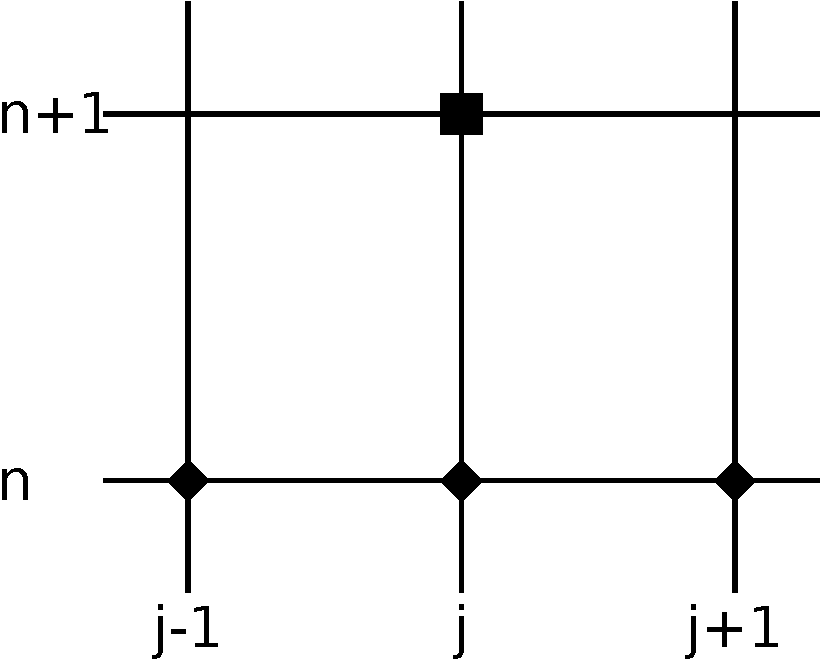
\includegraphics[width=2.5in]{expstencil}
\quad
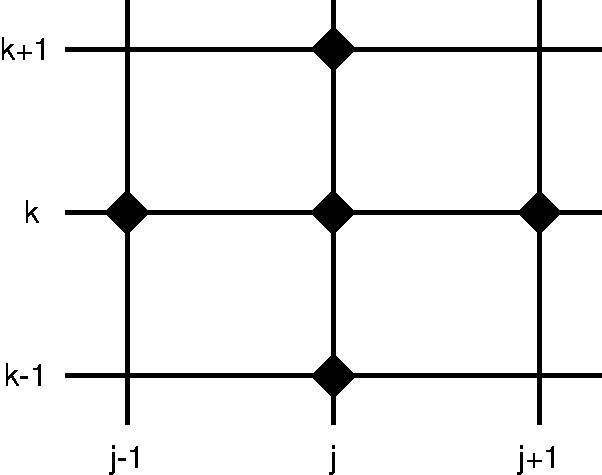
\includegraphics[width=2.5in]{exp2dstencil}

FIXME: identify schemes
\end{center}


implementation

\minput{heat}

\begin{itemize}
\item solves $u_t = D(u_{xx} + u_{yy})$ on square $-1 < x < 1$, $-1 < y < 1$
\item uses gaussian initial condition: $u_0(x,y) = e^{-30 r^2}$
\item uses ``colon notation'' to remove loops over spatial variables
\item \texttt{>>  heat(1.0,30,30,0.001,20)}

approximates $u$ on $30\times 30$ spatial grid, with $D=1$ and $N=20$ steps of $\Delta t = 0.001$
\end{itemize}


the look of success

\begin{itemize}
\item solving $u_t = u_{xx} + u_{yy}$ on $30\times 30$ grid
\end{itemize}


\begin{center}
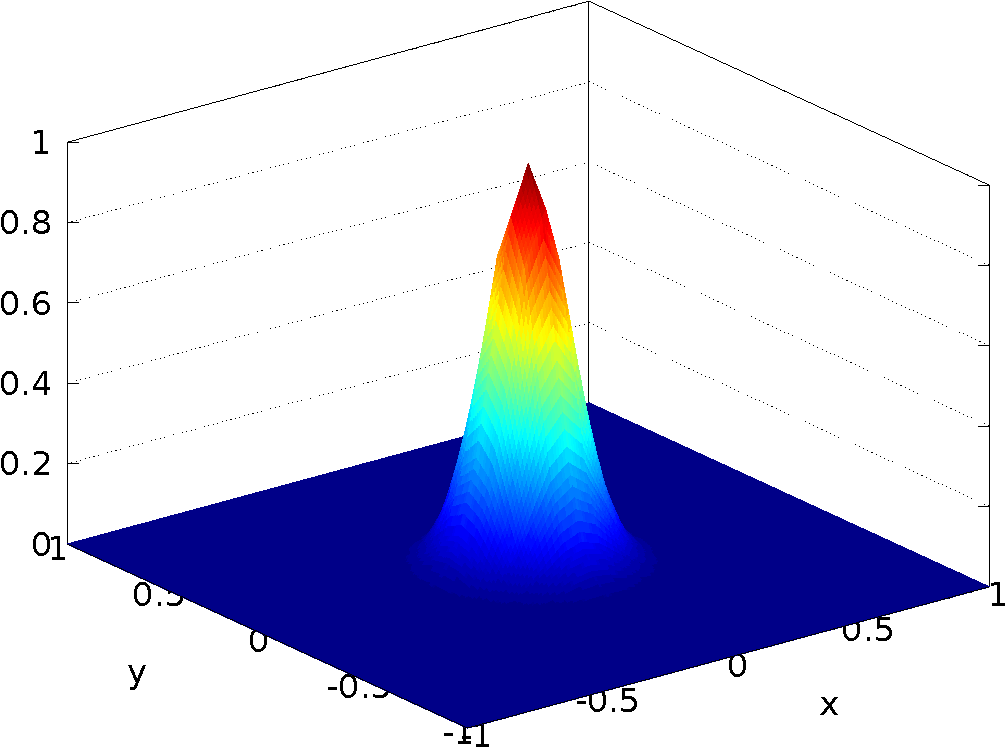
\includegraphics[width=2.5in]{initialheat}
\quad
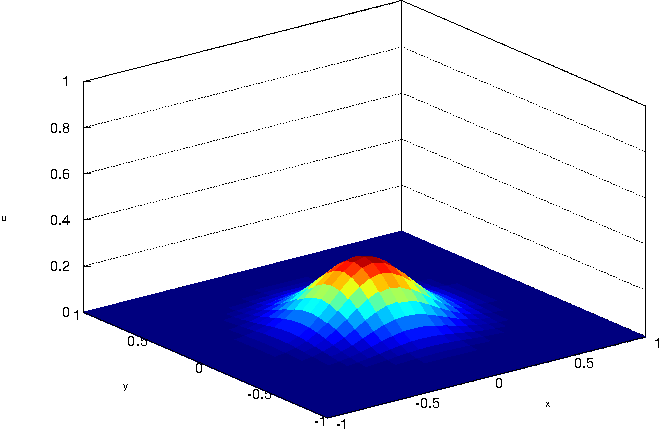
\includegraphics[width=2.5in]{finalheat}

initial condition $u(0,x,y)$ \qquad approximate solution $u(t,x,y)$ at $t=0.02$ with $\Delta t=0.001$
\end{center}


the look of instability

\begin{itemize}
\item both figures are from solving $u_t = u_{xx} + u_{yy}$ on the same space grid, but with slightly different time steps
\end{itemize}

\begin{center}
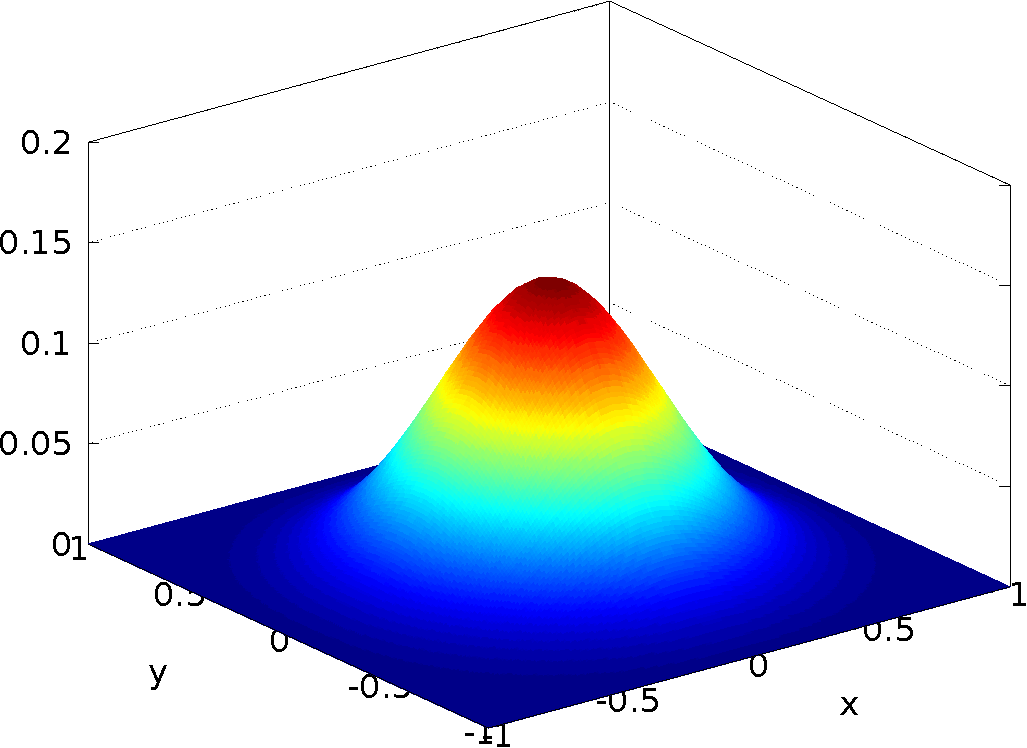
\includegraphics[width=2.5in]{stability}
\quad
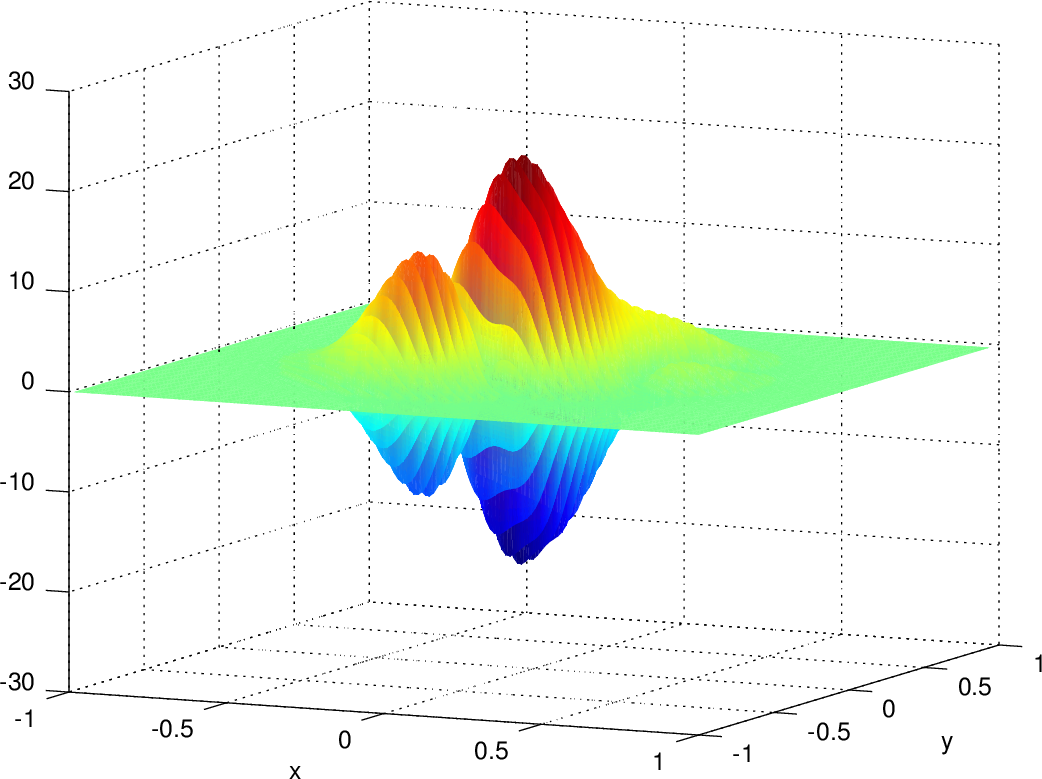
\includegraphics[width=2.5in]{instability}

%$D=1,\Delta t = 0.00064286,\Delta x = \Delta y = 0.04$ so
%$D=1,\Delta t = 0.001,\Delta x = \Delta y = 0.04$ so
$\frac{D\Delta t}{\Delta x^2}= 0.402$ \quad
$\frac{D\Delta t}{\Delta x^2}= 0.625$
\end{center}

avoid the instability

\begin{itemize}
\item recall 1D explicit scheme had the form 
	$$u_j^{n+1} = \nu u_{j+1}^n + (1 - 2 \nu) u_j^n + \nu u_{j-1}^n$$
\item thus the new value $u_j^{n+1}$ is an \emph{average} of the old values, \emph{if the middle coefficient is positive}:
	$$1 - 2 \nu \ge 0 \quad \iff \quad  \frac{D\Delta t}{\Delta x^2} \le \frac{1}{2} \quad \iff \quad \Delta t \le \frac{\Delta x^2}{2 D}$$
\item averaging is always stable because averaged wiggles are always smaller than the original wiggles
\item \dots so this condition is a sufficient \emph{stability criterion}
\item so:

\begin{center}
\emph{the result was unstable because the time step was too big}
\end{center}
\end{itemize}

\textsl{adaptive} implementation: guaranteed stability

\mmess{heatadapt}

\begin{itemize}
\item same as \texttt{heat.m} except

\begin{center}
\emph{choose time step from stability criterion}
\end{center}
\end{itemize}

alternative instability fix: implicitness

\begin{itemize}
\item explicit scheme is only ``conditionally stable'', but there are methods which are stable for \emph{any} positive time step $\Delta t$
\end{itemize}

\begin{itemize}
\item an implicit scheme is \emph{Crank-Nicolson} $\longrightarrow$
\item Crank-Nicolson has smaller error too: $O(\Delta t^2,\Delta x^2)$
\end{itemize}

\begin{itemize}
\item \emph{but} you have to solve linear systems of equations to take each time step
\item \scriptsize Donald Knuth has advice for ice sheet modelers: \begin{quote}
\emph{We should forget about small efficiencies \dots: premature optimization is the root of all evil}.
\end{quote}
\end{itemize}

variable diffusivity and time steps

\begin{itemize}
  \item recall the analogy: \qquad (SIA) $\leftrightarrow$ (heat eqn)
  \item the SIA has a diffusivity which varies in space, so consider a more general heat equation:
  		$$u_t = F + \Div \left(D(x,y) \grad u\right)$$
  \item the explicit method is conditionally stable with the same time step restriction if we evaluate diffusivity $D(x,y)$ at \alert{staggered} grid points:
\begin{align*}
\Div \left(D(x,y) \grad u\right) &\approx \frac{D_{j+1/2,k}(u_{j+1,k} - u_{j,k}) - D_{j-1/2,k}(u_{j,k} - u_{j-1,k})}{\Delta x^2} \\
	&\qquad + \frac{D_{j,k+1/2}(u_{j,k+1} - u_{j,k}) - D_{j,k-1/2}(u_{j,k} - u_{j,k-1})}{\Delta y^2}
\end{align*}
\end{itemize}

\begin{center}
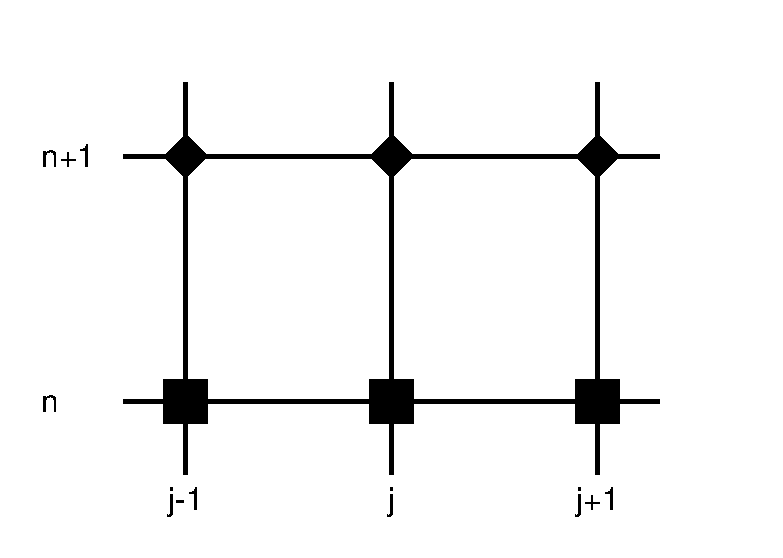
\includegraphics[width=1.8in]{cnstencil}
\quad
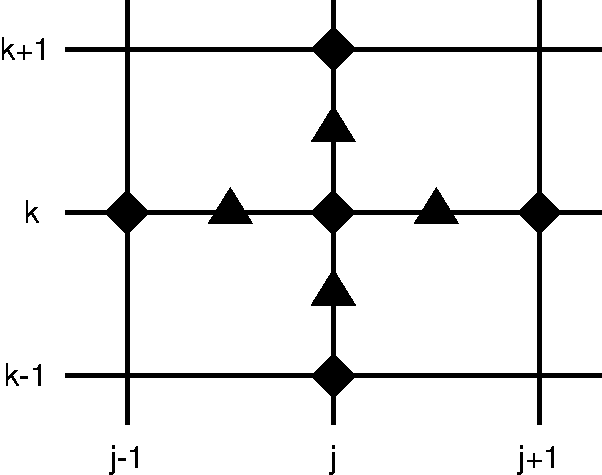
\includegraphics[width=1.8in]{diffstencil}
\quad
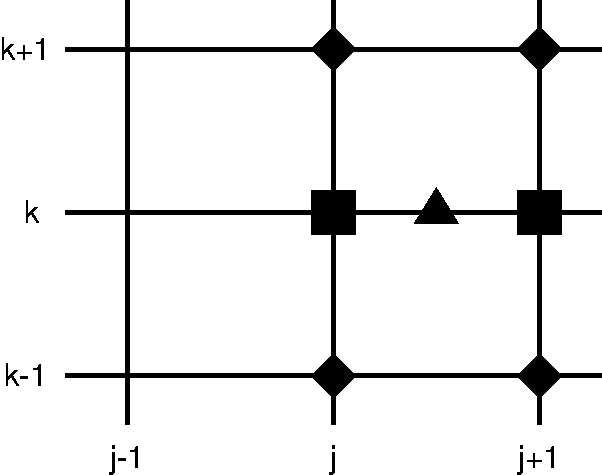
\includegraphics[width=1.8in]{mahaffystencil}
\end{center}

in stencil at right:
\begin{itemize}
\item[] diamonds: $u$
\item[] triangles: $D$
\end{itemize}


general diffusion equation code

\minput{diffusion}

\begin{itemize}
\item solves abstract diffusion equation $u_t = \Div \left(D(x,y)\, \grad u\right)$
\item user supplies diffusivity on staggered grid
\end{itemize}


\subsection{solutions}

exact solution of heat equation

\begin{itemize}
\item before getting to ice flow, one more heat equation topic \dots
\item the simple heat equation in 1D with constant diffusivity $D>0$ is:
	$$u_t = D u_{xx}$$
\item many \emph{exact} solutions to the heat equation are known, but I'll show the ``Green's function''
\item \dots also known as ``fundamental solution'' or ``heat kernel''
\item it starts at time $t=0$ with a ``delta function'' of heat at the origin $x=0$ and then it spreads out over time
\item we find it by a method which generalizes to the SIA
\end{itemize}

Green's function of heat equation

\begin{itemize}
\item the solution is ``self-similar'' over time
\item as time goes it changes shape by
  \begin{itemize}
  \item[$\circ$] shrinking the output (vertical) axis and
  \item[$\circ$] lengthening the input (horizontal) axis
  \end{itemize}
\item \dots but otherwise it is the same shape
\item the integral over $x$ is independent of time
\end{itemize}

\begin{center}
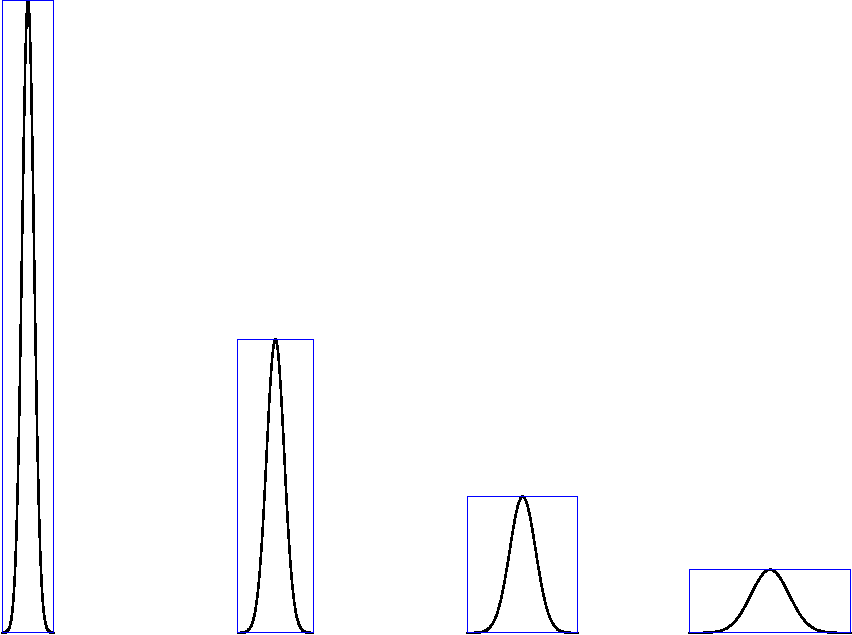
\includegraphics[width=3.0in]{heatscaling}

\emph{increasing time} $\to$
\end{center}

similarity solutions

\begin{itemize}
\item Green's function of heat equation in 1D is
	$$u(t,x) = C\, t^{-1/2} e^{-x^2/(4Dt)}$$
\item ``similarity'' variables for 1D heat equation are
	$$s \stackrel{\text{\emph{input scaling}}}{\phantom{\Big|}=\phantom{\Big|}} t^{-1/2} x, \qquad u(t,x) \stackrel{\text{\emph{output scaling}}}{\phantom{\Big|}=\phantom{\Big|}} t^{-1/2} \phi(s)$$
\end{itemize}

\begin{itemize}
\item \emph{historical note}:  in 1905 Einstein saw that the average distance traveled by particles in thermal motion scales like $\sqrt{t}$, so $s = t^{-1/2}x$ is an invariant
\end{itemize}

\begin{center}
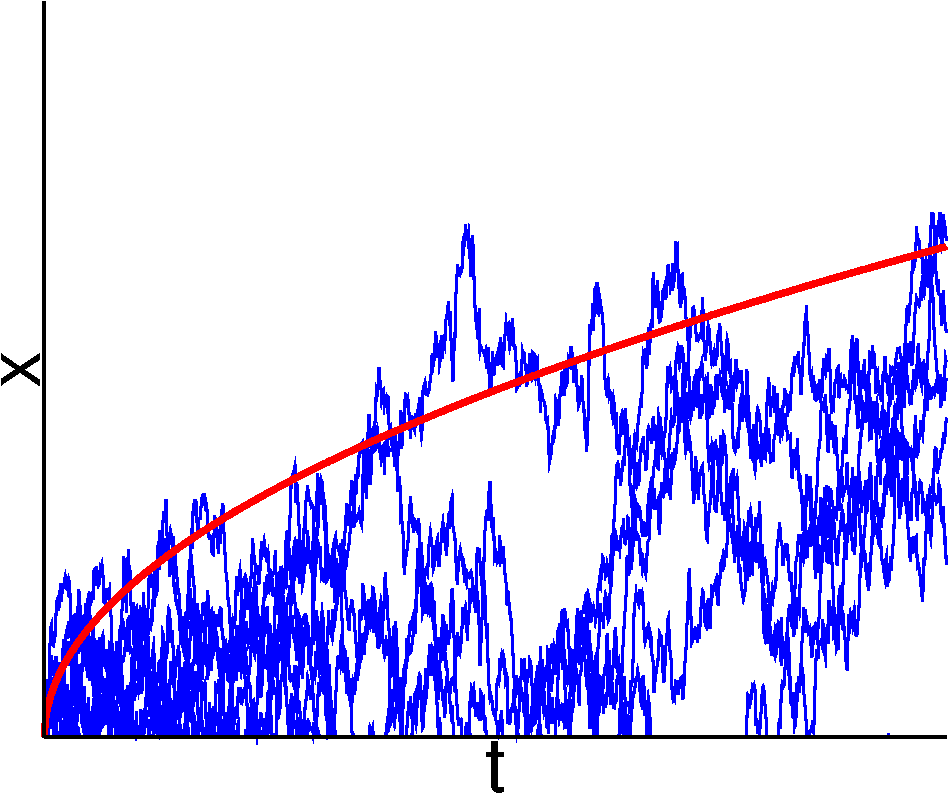
\includegraphics[width=3.0in]{brownian}
\end{center}

\subsection{solving the SIA}

similarity solution to SIA

\begin{itemize}
\item jump forward to 1981
\item P.~Halfar found the similarity solution of the SIA in the case of flat bed and no surface mass balance \nocite{Halfar81,Halfar83}
\item Halfar's 2D solution for Glen flow law with $n=3$ has scalings
   $$H(t,r)=t^{-1/9} \phi(s), \qquad s = t^{-1/18} r$$
\item \dots so the diffusion of ice really slows down as the shape flattens out!
\end{itemize}

Halfar solution to the SIA: the movie

%\animategraphics[autoplay,loop,height=7.0cm]{4}{anim/halfar}{0}{26}

frames from $t=4$ months to $t = 10^6$ years, equal spaced in \emph{exponential} time

Halfar solution to the SIA: the formula

\begin{itemize}
\item for $n=3$ the solution formula is:
  $$H(t,r) = H_0 \left(\frac{t_0}{t}\right)^{1/9} \left[1 - \left(\left(\frac{t_0}{t}\right)^{1/18} \frac{r}{R_0}\right)^{4/3}\right]^{3/7}$$
\item the ``characteristic time'' is
  $$t_0 = \frac{1}{18 \Gamma} \left(\frac{7}{4}\right)^3 \frac{R_0^4}{H_0^{7}}$$
if $H_0$, $R_0$ are central height and ice cap radius at $t=t_0$
\item you choose $H_0$ and $R_0$ and then determine $t_0$
\item it is a simple formula to use for verification!
\end{itemize}

is the Halfar solution \emph{good for any modeling}?

\begin{itemize}
\item John Nye and others (2000)\nocite{NyeIcarus2000} compared the long-time consequences of different flow laws for the South Mars Polar Cap
\item they evaluated $\text{CO}_2$ ice and $\text{H}_2\text{O}$ ice softness parameters
\item \dots by comparing the long-time behavior of the corresponding Halfar solutions
\item conclusions:
  \begin{quote}
  \dots none of the three possible [$\text{CO}_2$] flow laws will allow a 3000-m cap, the thickness suggested by stereogrammetry, to survive for $10^7$ years, indicating that the south polar ice cap is probably not composed of pure $\text{CO}_2$ ice \dots the south polar cap probably consists of water ice, with an unknown admixture of dust.
  \end{quote}
\end{itemize}

on ``degenerate'' diffusivity

\begin{itemize}
\item recall that the SIA is
	$$H_t = M + \Div \left(D\, \grad h \right) \quad \text{where} \quad D = \Gamma H^{n+2} |\grad h|^{n-1}$$
\item thus the diffusivity ``degenerates'', $D \to 0$, when either $H\to 0$ or $\grad h \to 0$
\item summary:
\begin{tabular}{l|c|c}
 & why $D\to 0$ & so what? \\ \hline
domes    & $\grad h \to 0$ & \begin{tabular}{c}
$H$ and $\grad h$ are continuous \\ but $\grad^2 h$ is singular
\end{tabular} \\ \hline
margins  & $H \to 0$       & \begin{tabular}{c}
$H$ is continuous \\ but $\grad h$ is singular
\end{tabular}
\end{tabular}
\item in terms of numerical error, margin is worse than dome
\item degenerate diffusion equations are automatically free boundary problems
\end{itemize}

computing diffusivity in SIA

\begin{itemize}
\item for numerical stability we compute $D = \Gamma H^{n+2} |\grad h|^{n-1}$ on the staggered grid
\item various schemes proposed \small (Mahaffy, 1976\nocite{Mahaffy}; van der Veen 1999\nocite{vanderVeen}; Hindmarsh and Payne 1996\nocite{HindmarshPayne})
\item all schemes involve
  \begin{itemize}
  \item[$\circ$] averaging $H$
  \item[$\circ$] differencing $h$
  \item[$\circ$] in a ``balanced'' way, for better accuracy,
  \end{itemize}
to get the diffusivity on staggered grid

\item Mahaffy stencil shown in previous figure
\end{itemize}


SIA implementation: flat bed case

\minputtiny{siaflat}

verification of numerical ice flow codes

\begin{itemize}
\item how do we make sure an \emph{implemented} numerical scheme is correct?
  \begin{itemize}
  \item[$\circ$] \emph{technique} 1: don't make any mistakes
  \item[$\circ$] \emph{technique} 2: compare your model with others, and hope that the outliers are the ones with errors
  \item[$\circ$] \emph{technique} 3: build-in a comparison to an exact solution, and actually measure the numerical error \alert{$=$ verification}
  \end{itemize}
\item where to get exact solutions for ice flow models?
  \begin{itemize}
  \item[$\circ$] textbook: Greve and Blatter (2009)\nocite{GreveBlatter2009}
  \item[$\circ$] similarity solutions to SIA (Halfar 1983\nocite{Halfar83}; Bueler et al 2005\nocite{BLKCB})
  \item[$\circ$] manufactured solutions to thermo-coupled SIA (Bueler et al 2007\nocite{BBL})
  \item[$\circ$] flowline and cross-flow SSA solutions (van der Veen, 1985; Schoof, 2006)\nocite{SchoofStream,vanderVeen85}
  \item[$\circ$] flowline Blatter solutions (Glowinski and Rappaz 2003)\nocite{GlowinskiRappaz}
  \item[$\circ$] flowline Stokes solutions for constant viscosity (Ladyzhenskaya 1963\nocite{Ladyzhenskaya}, Balise and Raymond 1985\nocite{BaliseRaymond1985})
  \item[$\circ$] manufactured solutions to the Stokes equations (Sargent and Fastook 2010; Jouvet and Rappaz 2011)\nocite{JouvetRappaz2011,SargentFastook2010}
  \end{itemize}
\end{itemize}

verifying SIA code vs Halfar

\begin{verbatim}
octave:40> verifysia(20)
average abs error            = 22.310
maximum abs error            = 227.849
octave:41> verifysia(40)
average abs error            = 9.490
maximum abs error            = 241.470
octave:42> verifysia(80)
average abs error            = 2.800
maximum abs error            = 155.796
octave:43> verifysia(160)
average abs error            = 1.059
maximum abs error            = 109.466
\end{verbatim}


demonstrate robustness

see \texttt{roughice.m}, which calls \texttt{siaflat.m} after setting-up the nasty initial state at left:

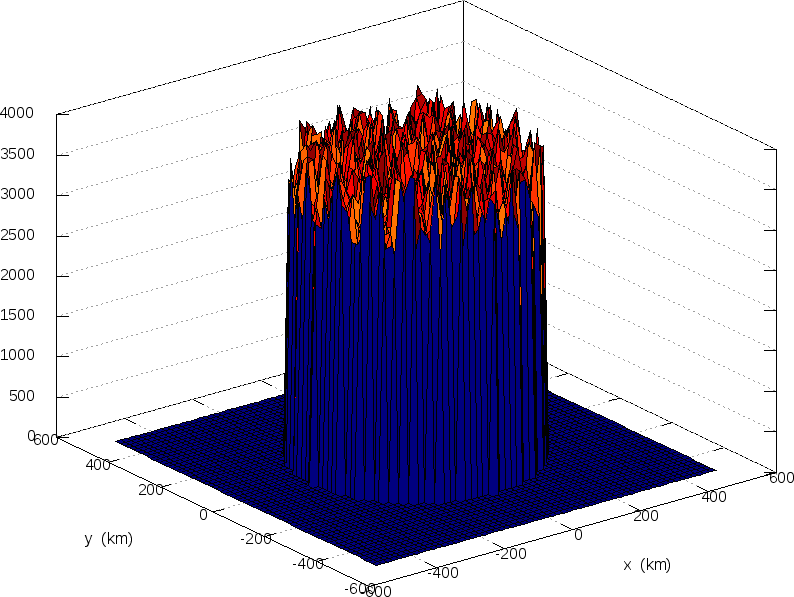
\includegraphics[width=2.5in]{roughinitial}
\quad
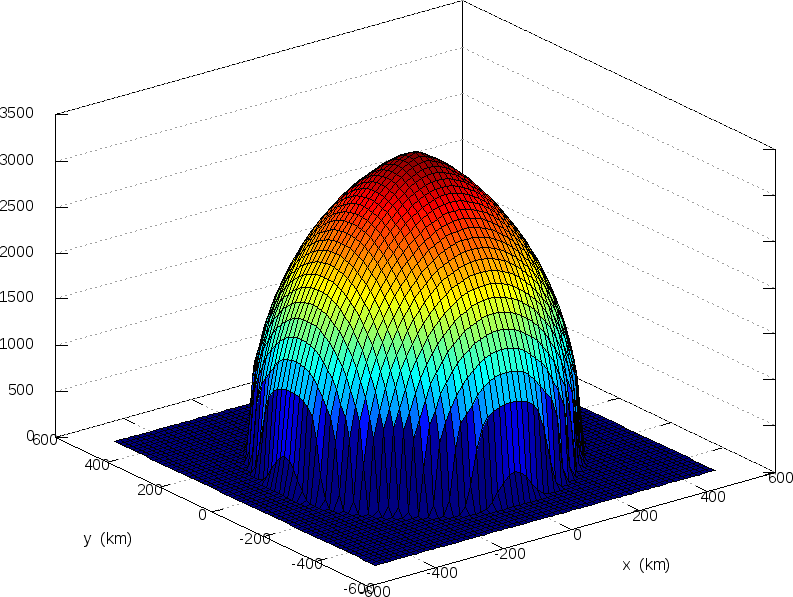
\includegraphics[width=2.5in]{roughfinal}



model the Antarctic ice sheet

\begin{itemize}
\item with careful-but-small modifications of \texttt{siaflat.m}, which make a good exercise:
  \begin{itemize}
  \item[$\circ$] observed accumulation as surface mass balance,
  \item[$\circ$] allow non-flat bed (so $H\ne h$),
  \item[$\circ$] differentiate the surface correctly where floating, and
  \item[$\circ$] calve at current calving front location
  \end{itemize}
here are results from this \emph{toy} Antarctic flow model
\item a 2000 model year run on a $\Delta x=50$ km grid; runtime a few seconds
\end{itemize}

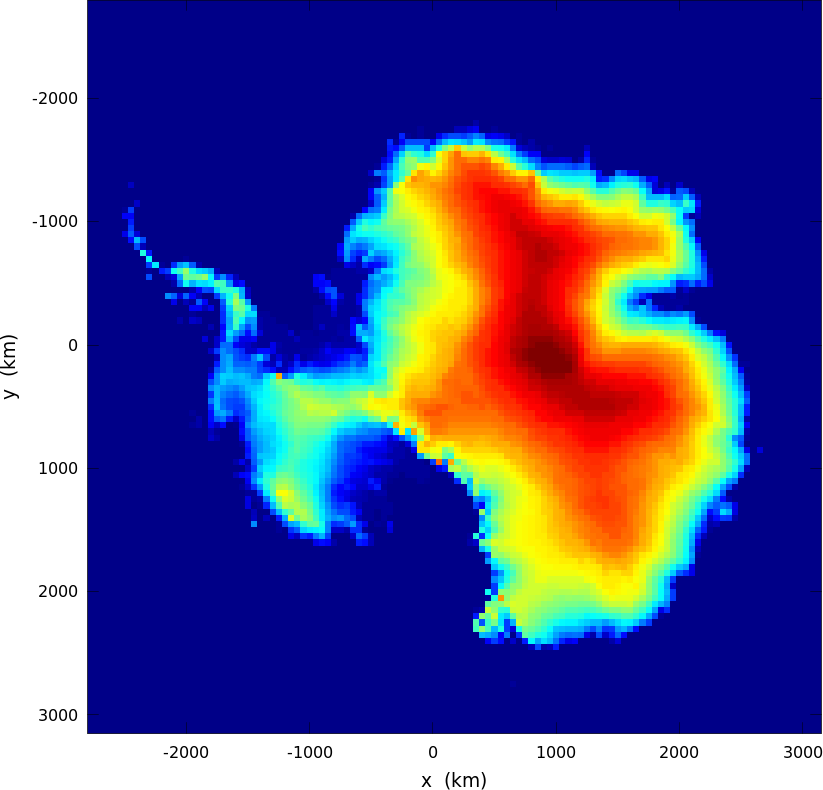
\includegraphics[width=2.5in]{antinitial}
\quad
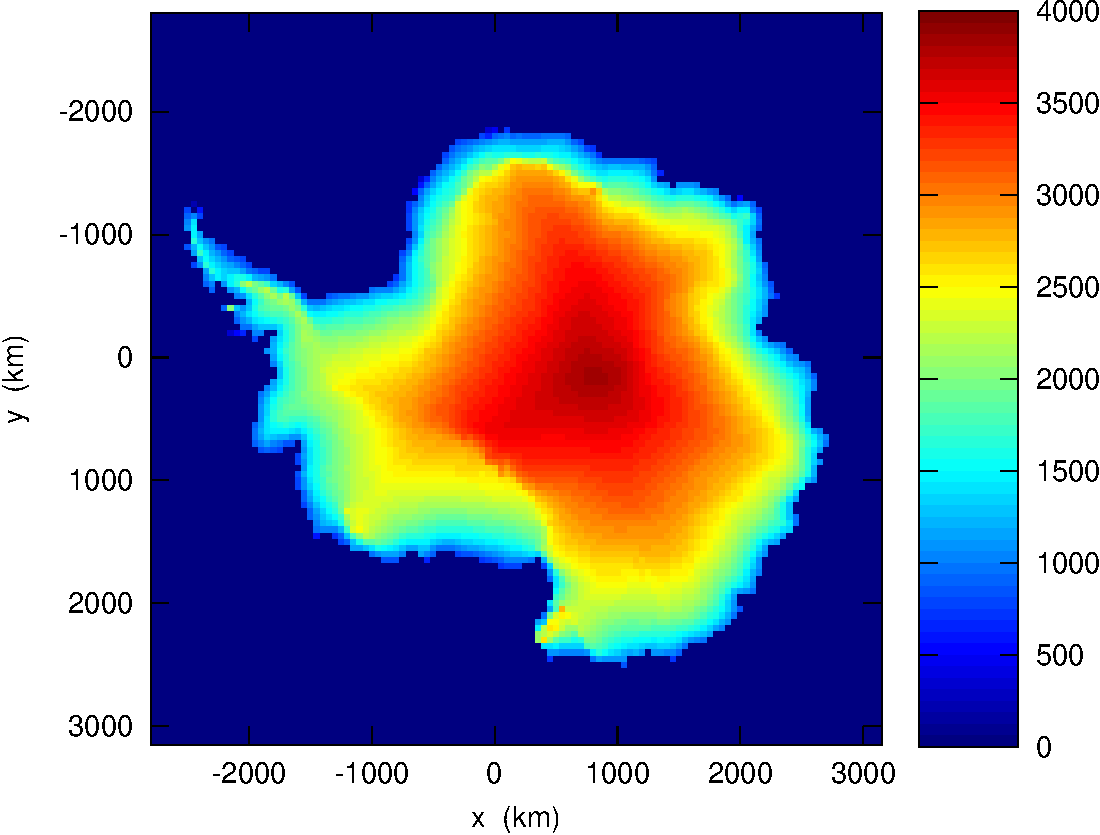
\includegraphics[width=2.5in]{antfinal}

final comments on SIA: origin and rigor

where does the ``shallow ice approximation'' come from?:

\begin{itemize}
\item historically, Fowler and Larson (1978)\nocite{FowlerLarson1978}, Morland and Johnson (1980)\nocite{MorlandJohnson}, and Hutter (1983)\nocite{Hutter} \dots thus recent
\item logically, by a ``small-parameter argument'', based on a small depth-to-width ratio, from the more complete Stokes model for slow ice flow
\item more precisely, by using the small aspect ratio \, $\eps = [H]/[L]$ \, of ice sheets to scale the Stokes model to see which terms make small contributions
\end{itemize}

%         References
\clearpage\newpage
\bibliography{ice_bib}
\bibliographystyle{siam}

\end{document}